\documentclass[spanish]{udpreport}
\usepackage[utf8]{inputenc}
\usepackage[spanish]{babel}

% Podemos establecer el logo de alguna entidad o dejar el de la UDP (defecto)
%\setlogo{EITFI}

\title{Informe Laboratorio I \\ Redes de Datos}
\author{Arturo Mantinetti \\ Manuel Tobar \\ Diego Vilches \\ Tercer Amigo}
\email{arturo.mantinetti@mail.udp.cl \\ manuel.tobar@mail.udp.cl
	\\ diego.vilches@mail.udp.cl \\ tercer.amigo@mail.udp.cl}
	
\profesor{Profesor \\ Jaime Álvarez}
\ayudante{Ayudante \\ Maximiliano Vega}


\date{29 de Marzo de 2016}

% Además podemos establecer la facultad y escuela
% los valores por defecto son los siguientes:
%\udpschool{Escuela de Informática y Telecomunicaciones}
%\udpfaculty{Facultad de Ingeniería}
%\udpuniversity{Universidad Diego Portales}

\begin{document}
\maketitle

\tableofcontents

\chapter{Introducción}

Este laboratorio consta de tres actividades. La primera consiste en identificar todos los equipos que están conectados a la red, los switch de la topología, el hardware de red utilizado, tomando en cuenta su marca y modelo, el tipo de cableado ocupado, junto a sus características y por último el patch panel. La segunda actividad consiste en obtener la información de los equipos ya mencionados. Ocupando el terminal, se tiene que obtener la IP y la MAC de cada equipo, todo esto con el objetivo de obtener una mayor comprensión de la red. Finalmente, con todos los datos recopilados en las dos actividades anteriores, se procede a generar el diagrama de un mapa de red, en el cual, esta se debe ver representada,  especificando todos los datos recopilados durante la experiencia.


\chapter{Contenido}

\section{Topologia y Hardware}
El tipo de topología presente en esta experiencia es de arbol, ya que la red pasa desde el siwtch a todos los host, que en este caso, serían todos los equipos de la sala.
\\
 % Aca ponemos el tipo de hardware del switch, etc...
 
\setlength{\parindent}{0.5cm} Con respecto a al hardware de los equipos, el switch es de marca Cisco y el modelo es Catalyst 2960. Entre sus características se encuentran que posee 24 puertos de 10/100, en los cuales se encuentran conectados los equipos de la sala, y dos puertos gigabit. Por otra parte, todo el cableado de los equipos es de categoría 5e y de par directo.
\begin{center}
	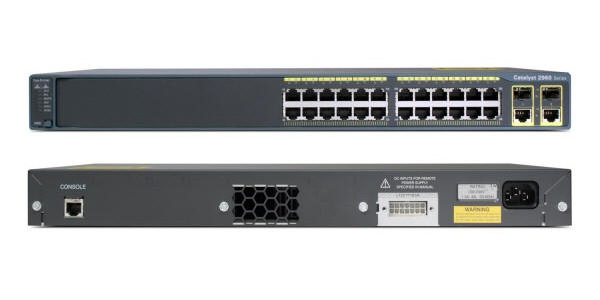
\includegraphics[scale=.37]{images/switch.png}
\end{center}
  
\section{Datos de equipos}
% Aca poner macs e ips and shit...
Ocupando la consola de los equipos, se pueden recopilar las IPs y las MAC de los equipos. La IP es el numero que identifica al equipo, en este caso dentro dentro de la red LAN, esta utiliza el protocolo IP dentro del modelo TCP/IP, de tal forma la red saber de que equipo proviene cada trafico, esta está definida por cuatro rangos de 256 valores cada uno en el caso de IPv4. Por otro lado la MAC es el identificador físico de la tarjeta de red del equipo, este no cambia cuando uno se conecta a otra red LAN a diferencia de la dirección IP, la dirección MAC está definida por 6 pares hexadecimales, donde los primeros tres pares son identificador del fabricante y los últimos tres son del controlador de la tarjeta de red.
\\

\setlength{\parindent}{0.5cm} Al analizar las IPs de los equipos, se puede observar que todas son muy similares, defiriendo solamente el ultimo octeto de esta, siendo asignadas de manera estática dentro de las configuraciones de las interfaces de red de Ubuntu. Esto implica que todos los equipos se encuentran en el mismo rango de red. Por otro lado, también se puede ver que todos los equipos tienen los mismos tres primeros pares de la MAC, lo que implica que las tarjetas de red de estos proceden del mismo fabricante.



\pagebreak
\section{Mapa de Red}
En esta sección se puede observar las características de los equipos y el hardware, además de las conexiones de la red en si. 
\begin{center}
	\includegraphics[scale=.37]{images/mapa_red.png} 
\end{center}

\listoffigures

\chapter{Conclusión}

A partir de la información que recopilamos logramos identificar desde el hardware de los equipos del laboratorio hasta la topología presente. Esto nos permitió hacer una correcta representación de cómo está estructurado el laboratorio. Por medio de las direcciones IP  supimos que todos los equipos trabajan dentro de un mismo rango de red y gracias a las direcciones MAC averiguamos de qué fabricante es el modelo de las tarjetas de red que todos los equipos comparten, ademas el tipo de cableado nos dio una idea de la capacidad de transferencia de información entre los equipos. 

\\

\setlength{\parindent}{0.5cm} Lo anterior junto con otra información nos permitió hacer un mapa que muestra todos los elementos del laboratorio y como estos interactúan entre ellos pudiéndose incluso recrear con precisión el ambiente de red del laboratorio basándose en nuestra información. Esta experiencia nos permitió aprender a reconocer como está organizado un ambiente de red, saber identificar los elementos que la componen y como estos interactúan entre si.

\end{document}
